\section{INTRODUCTION}

Autonomous robots are increasingly deployed in human-populated environments for diverse applications, from service robotics to delivery systems and assistive technologies. As robots become more prevalent in social spaces, developing navigation strategies that respect human social dynamics has emerged as a critical challenge \cite{CHARALAMPOUS201785, pandey2017mobile}. Socially compliant navigation extends beyond simple collision avoidance—it requires robots to understand and respect the implicit social contracts that govern human movement patterns. While early approaches treated humans as dynamic obstacles \cite{fox1997dynamic}, research has progressively incorporated social awareness, from preventing deadlocks in crowds \cite{trautman2015robot} to encoding basic social norms for more natural robot behaviors \cite{bera2017sociosense}. Yet despite these advances, most existing methods model humans as isolated individuals, overlooking a fundamental aspect of human crowd dynamics: the formation and movement of social groups. 

% \SR{Such violations induce psychological discomfort and stress in humans even when no physical danger is present, directly impacting human acceptance and willingness to share spaces with robots~\cite{gao2022evaluation}.}

\begin{figure}[!t]
\centering
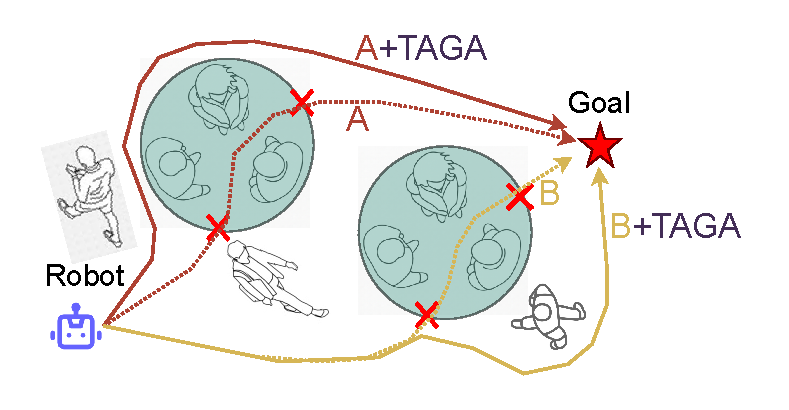
\includegraphics[width=4in]{figures/ntheme.pdf}
\vspace{-23pt}
 
\caption{Comparison of baseline and TAGA (group-aware) robot navigation in a multi-group environment. The \textcolor{blue}{robot} navigates toward the goal \textcolor{red}{$\bigstar$} through human groups (\textcolor[HTML]{70B0A8}{teal circles}) and individuals. Baseline navigation methods \textcolor[HTML]{AE4132}{A} and \textcolor[HTML]{D6B656}{B} (dotted lines) cut directly through group spaces, violating social norms (marked by \textcolor{red}{×}). In contrast, TAGA-enhanced paths \textcolor[HTML]{AE4132}{A}+TAGA and \textcolor[HTML]{D6B656}{B}+TAGA (solid lines) guide the robot around groups, respecting group boundaries while efficiently reaching the goal. \SR{I changed the caption. Some points were not clear in the previous one. Feel free to revise this one if required.}}
\vspace{-15pt} 
\label{fig-env-theme}
\end{figure}

% \caption{Comparison of baseline and TAGA (group-aware) robot navigation in a multi-group environment. The robot (blue icon, left) navigates toward its goal (red star, right) through a scene with two human groups (\textcolor[HTML]{70B0A8}{teal circles}) and several individuals (gray figures). Baseline navigation methods \textcolor[HTML]{AE4132}{A} and \textcolor[HTML]{D6B656}{B} (shown as dotted lines) cut directly through group spaces, violating social norms (marked by \textcolor{red}{×}). In contrast, TAGA-enhanced paths \textcolor[HTML]{AE4132}{A}+TAGA and \textcolor[HTML]{D6B656}{B}+TAGA (solid lines) guide the robot around groups, respecting group boundaries while efficiently reaching the goal.   \SR{I changed the caption. Some points were not clear in the previous one. Feel free to revise this as well.}}

% 

% \begin{figure}[!t]
% \centering
% 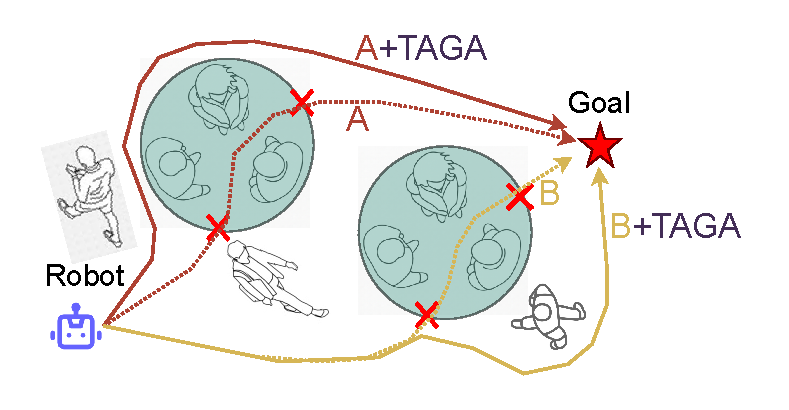
\includegraphics[width=4in]{figures/ntheme.pdf}
% \vspace{-23pt}
% \caption{
% % Comparison of robot navigation with and without TAGA integration. (a) Traditional environment without group modeling, where robots navigate toward goals without considering human group formations. (b) Our enhanced environment with detected human groups (bounded by dotted black circles). Existing navigation frameworks (labeled A and B) frequently intrude into these groups, while their TAGA-enhanced versions (A+TAGA and B+TAGA) generate paths that respect group boundaries while maintaining effective navigation toward goals. 

% % Comparison of baseline and TAGA (group-aware) paths in a multi-group environment. 
% % Baseline paths of \textcolor[HTML]{AE4132}{A} and \textcolor[HTML]{D6B656}{B} (shown as dotted lines) occasionally cross group boundaries, indicating violations of group constraints (highlighted by small `\textcolor{red}{×}' markers). In contrast, TAGA paths (\textcolor[HTML]{AE4132}{A}+TAGA and \textcolor[HTML]{D6B656}{B}+TAGA) remain fully within their assigned regions, demonstrating improved group compliance and cooperative navigation.

% Comparison of baseline and TAGA (group-aware) robot navigation in a multi-group environment. The robot (blue icon, left) navigates toward its goal (red star, right) through a scene with two human groups (\textcolor[HTML]{B0D1CB}{teal circles}) and several individuals (gray figures). Baseline navigation methods \textcolor[HTML]{AE4132}{A} and \textcolor[HTML]{D6B656}{B} (shown as dotted lines) cut directly through group spaces, violating social norms (marked by \textcolor{red}{×}). In contrast, TAGA-enhanced paths \textcolor[HTML]{AE4132}{A}+TAGA and \textcolor[HTML]{D6B656}{B}+TAGA (solid lines) guide the robot around groups, respecting group boundaries while efficiently reaching the goal.

% % \SR{The current two-panel design may confuse the reviewers. Panels (a) and (b) show different spatial arrangements of humans, which undermines the comparative purpose of the figure. Instead, redesign this as a single panel showing:
% % One environment with detected human groups (visualized with shaded regions or dotted boundaries)
% % Path A (group-unaware) - clearly intruding through groups,
% % Path B (group-unaware) - clearly intruding through groups,
% % Path A+TAGA (group-aware) - avoiding/respecting group boundaries, and
% % Path B+TAGA (group-aware) - avoiding/respecting group boundaries.
% % Use different colors and distinct line styles for each path with a clear legend. Make it visually obvious where group-unaware paths violate social norms - show paths cutting through group centers, contrasted with TAGA paths navigating around them.}
% } 
% % \SR{I think it's okay now. Consider adding small "×" markers where baseline paths intersect group boundaries to make violations more obvious. Write a good caption for the figure.\UT{Did it}}
% \vspace{-15pt} 
% \label{fig-env-theme}
% \end{figure}

Human crowds naturally organize into groups—families walking together, friends in conversation, colleagues moving between meetings—that create distinct spatial and social patterns \cite{moussaid2010walking}. These group formations significantly influence crowd flow and establish implicit boundaries that should be respected during navigation. When robots fail to recognize these group structures, they exhibit behaviors that humans perceive as rude or unsafe, such as cutting between conversing friends or passing through family clusters. Traditional navigation methods, including reactive approaches like Optimal Reciprocal Collision Avoidance (ORCA) \cite{orca} and Social Force models \cite{helbing1995social}, as well as learning-based systems \cite{liu2020decentralized, liu2023intention}, treat each person independently. Consequently, robots using these methods may achieve collision-free navigation while still violating social expectations by intruding into group spaces. Such violations induce psychological discomfort and stress in humans even when no physical danger is present, directly impacting human acceptance and willingness to share spaces with robots~\cite{gao2022evaluation}.

% \SR{The third paragraph (Recent attempts to....) needs revision to provide a comprehensive overview of related work. A strong introduction paragraph on prior work should: (1) introduce multiple relevant prior works on group-aware navigation, (2) systematically identify their limitations, and (3) complete the thought about the critical gap in real-time group detection. Currently, you cite only [11], which makes the literature review appear thin and incomplete. You have cited several other relevant group-aware methods in Section III—some of these should be briefly introduced here to demonstrate breadth of understanding.}

% \SR{Why completing the real-time group detection gap is essential:
% Your work makes a fundamental claim: TAGA uses DBSCAN for real-time group detection from observable features rather than assuming pre-labeled group membership. However, if you don't explicitly establish that existing methods assume perfect group knowledge and that this is a critical flaw, reviewers won't understand why your detection approach is a contribution. They'll wonder: "Why not just use ground-truth labels like prior work?"}

% Recent attempts to incorporate group awareness into robot navigation have shown promise but remain limited in scope. Katyal et al. \cite{group-aware} introduced group modeling using convex hulls, treating groups as unified entities moving in consistent directions. However, this approach struggles with the diversity of real-world group behaviors—static conversation circles, dynamically forming clusters, and groups with varying internal structures. Furthermore, their method relies on reinforcement learning with group-specific penalties, requiring retraining for different environments and lacking the flexibility to integrate with existing navigation systems. 

% \SR{Check the following revised para}

Recent attempts to incorporate group awareness into robot navigation have shown promise but face significant limitations. Katyal et al.~\cite{group-aware} introduced group modeling using convex hulls, treating groups as unified entities moving in consistent directions. However, this approach struggles with diverse real-world scenarios—such as static conversation circles, dynamically splitting clusters, and groups with non-uniform velocities. Their reinforcement learning approach with group-specific penalties requires retraining for different environments and cannot easily integrate with existing navigation systems. Similarly, geometric approaches like SEAN 2.0~\cite{tsoi2023sean} model F-formations with predefined spatial zones but require rigid formation parameters that don't adapt to dynamic group changes, while learning-based methods like SNGNN~\cite{wang2023learning} and CoMet~\cite{nishimura2022comet} need extensive training on group-labeled datasets.

% Most critically, current approaches often assume perfect knowledge of group membership, rather than addressing the challenge of real-time group detection in dynamic crowds.



\UT{Try to address the 1st review of reviwer 31281}Most critically, current approaches often assume perfect knowledge of group membership, rather than addressing the challenge of real-time group detection in dynamic crowds. In practical robot deployments, group membership is not observable---robots can only perceive individual positions and velocities through their sensors. They must infer group structure dynamically as people cluster, split, and reform. \SR{For instance, in Figure~\ref{fig-env-theme}, our proposed system intelligently distinguishes between an individual whose velocity is diverging from a nearby group (the person near the left group, moving away from it) versus an individual whose velocity is converging with a group (the person near the right group, moving toward it). In the former case, TAGA allows passage between the individual and group; in the latter, it treats them as a collective unit to navigate around.} Methods like~\cite{group-aware} that rely on pre-labeled group information or~\cite{tsoi2023sean} that require predefined F-formation parameters sidestep this fundamental challenge, limiting their applicability in real-world scenarios where group composition changes continuously.


% Most critically, current approaches often assume perfect knowledge of group membership, rather than addressing the challenge of real-time group detection in dynamic crowds. In practical robot deployments, group membership is not observable---robots can only perceive individual positions and velocities through their sensors. They must infer group structure dynamically as people cluster, split, and reform (Figure~\ref{fig-env-theme}). \SR{Our proposed system addresses this by using observable motion cues---detecting whether individuals' velocities are diverging from or converging toward nearby groups---to make real-time group membership decisions.} Methods like~\cite{group-aware} that rely on pre-labeled group information or~\cite{tsoi2023sean} that require predefined F-formation parameters sidestep this fundamental challenge, limiting their applicability in real-world scenarios where group composition changes continuously.

% To address these limitations, we present a comprehensive framework for group-aware robot navigation that combines realistic group modeling with a modular avoidance strategy. 
% % Building upon the simulation environment from \cite{liu2023intention}, we introduce dynamic group behaviors including spatial clustering, leader-follower dynamics, and varying group formations.
% \SR{We evaluate our approach in an extended simulation environment based on \cite{liu2023intention} }that incorporates dynamic group behaviors including spatial clustering, leader-follower dynamics, and varying group formations. Our key contribution is TAGA (Tangent Action for Group Avoidance), a reactive navigation module that computes tangent trajectories around detected groups. Unlike previous learning-based approaches, TAGA operates as a plug-in enhancement that can augment any existing navigation method without retraining, activating only when groups are detected and seamlessly returning control to the base navigation policy afterward. \SR{ As illustrated in Figure~\ref{fig-env-theme}, baseline paths cut through group spaces while TAGA paths respect group boundaries through tangent navigation.}


\SR{Building on this dynamic detection capability, we present} TAGA (Tangent Action for Group Avoidance), a comprehensive framework for group-aware robot navigation that combines realistic group modeling with a modular avoidance strategy. \SR{We evaluate our approach in an extended simulation environment based on~\cite{liu2023intention}} that incorporates dynamic group behaviors including spatial clustering, leader-follower dynamics, and varying group formations. Unlike previous learning-based approaches, TAGA operates as a plug-in enhancement that can augment any existing navigation method without retraining, activating only when groups are detected and seamlessly returning control to the base navigation policy afterward. \SR{As illustrated in Figure~\ref{fig-env-theme}, baseline paths cut through group spaces, while TAGA paths respect group boundaries through tangent navigation.}

% Our study makes the following contributions:
% \begin{enumerate}
%     \item We develop an enhanced simulation framework that models both individual and group dynamics with realistic clustering behaviors, leader-follower patterns, and mixed crowd compositions, enabling comprehensive evaluation of navigation strategies in complex social environments.
    
%     \item We propose TAGA, a modular group avoidance mechanism that dynamically computes tangent trajectories around detected human groups. TAGA integrates with existing navigation frameworks without requiring modification or retraining, demonstrating consistent improvements across reactive and learning-based methods.
    
%     \item We introduce Group Collision Rate (GCR) as an independent evaluation metric that measures the percentage of time robots spend within group boundaries. GCR provides continuous assessment of group-aware behavior throughout navigation episodes, where the traditional metrics satisfy SR + CR + TR = 1 for terminal states only. \SR{The current phrasing—"independent evaluation metric" and "where the traditional metrics satisfy SR + CR + TR = 1 for terminal states only"—is confusing and suggests GCR is superior to or separate from traditional metrics, when in fact it's complementary. Readers may misinterpret "independent" as meaning GCR doesn't relate to navigation quality, or that traditional metrics are flawed for only working at terminal states.}

%     \item \SR{We introduce Group Collision Rate (GCR) as a continuous metric complementary to traditional terminal state metrics. GCR measures the percentage of navigation time spent within group boundaries and provides frame-by-frame assessment of social compliance throughout the entire navigation episode. Unlike SR (?), CR(?), and TR(?) that only capture episode outcomes, GCR enables fine-grained evaluation of group-aware behavior.}
    
%     \item We implement a hierarchical safety controller that ensures individual collision avoidance during group maneuvers, addressing critical safety concerns when navigating near both groups and individuals simultaneously. This controller maintains multiple safety zones with graduated responses to prevent collisions while executing tangent trajectories.
    
%     \item We conduct comprehensive benchmarking across diverse scenarios including dense groups, mixed populations (50\% individuals, 50\% in groups), and dynamic formations. By integrating TAGA with established methods including ORCA \cite{orca}, Social Force \cite{helbing1995social}, DS-RNN \cite{liu2020decentralized}, and AG-RL \cite{liu2023intention}, we demonstrate \UT{I will give numbers later}
%     reduction in group intrusions while maintaining or improving navigation success rates.
% \end{enumerate}


Our study makes the following key contributions:

\begin{enumerate}
    \item \textbf{Real-time group detection.}
    We develop a DBSCAN-based module that identifies human groups online from observable motion cues (position, velocity, proximity), without assuming pre-labeled group membership.
    The module dynamically detects, updates, and dissolves group formations as they evolve, addressing a fundamental gap in practical socially compliant navigation.

    \item \textbf{Group-aware tangent navigation (TAGA).}
    We propose TAGA, a modular group-avoidance mechanism that computes tangent trajectories around detected group boundaries while maintaining individual safety.
    TAGA integrates with existing reactive and learning-based navigation frameworks without retraining, acting as a plug-in layer that activates only when groups are present.

    \item \textbf{Hierarchical safety control.}
    We design a three-zone safety controller (critical, warning, comfort) that coordinates group-level tangent maneuvers with individual collision avoidance in dense, mixed-population scenarios.

    \item \textbf{Realistic crowd simulation benchmark.}
    We introduce a benchmark environment incorporating five empirically motivated modeling phases: individual speed variation (Weidmann 1992), dynamic group speed coupling (Moussaïd 2010), F-formations for static groups (Kendon 1990), leader--follower dynamics (Helbing \& Molnár 1995), and convex-hull group boundaries.
    This benchmark enables reproducible evaluation under crowd conditions that closely reflect real-world group behavior.

    \item \textbf{Continuous group compliance metric (GCR).}
    We introduce the \textit{Group Collision Rate (GCR)}, a continuous metric that quantifies the fraction of navigation time spent inside group boundaries, providing frame-level social compliance assessment complementary to terminal-state metrics (SR, CR, TR).

    \item \textbf{Cross-method empirical study revealing reactive--learning asymmetry.}
    We benchmark TAGA against reactive methods (ORCA~\cite{orca}, Social Force~\cite{helbing1995social}) and learning-based methods (DS-RNN~\cite{liu2020decentralized}, AG-RL~\cite{liu2023intention}, GARN), uncovering a consistent pattern: explicit group-awareness yields the largest gains for reactive methods, while highly optimized learned policies that have implicitly internalized group-avoidance behavior benefit less.
    This finding offers concrete guidance on when modular group-awareness provides the most practical value.
\end{enumerate}

% \section{INTRODUCTION}

% \SR{Autonomous robots are rapidly transitioning from controlled industrial settings to complex human-populated environments—hospitals, shopping malls, airports, office buildings, and public spaces—where they must navigate alongside people to perform service tasks, deliveries, and assistance. Despite decades of research and significant technological progress, fundamental challenges still prohibit the seamless deployment of autonomous robots in crowded public environments~\cite{mavrogiannis2023core}. The consequences of poor social navigation extend beyond inefficiency: robots' navigational behaviors—such as how they approach and pass people—can induce feelings of discomfort or stress in humans, even when they don't physically endanger anyone. Field deployments in shopping malls have documented failed robot approaches and highlighted the need for socially acceptable navigation when interacting with the public. Studies measuring human comfort show that participants rate their psychological comfort significantly lower under various robot approach patterns and speeds~\cite{gao2022evaluation}. These failures directly impact human acceptance and willingness to share spaces with robots—a critical barrier as society increasingly relies on robotic systems for essential services. As robots become more prevalent in our daily lives, developing navigation strategies that not only avoid collisions but actively respect human social norms has emerged as an essential requirement for successful human-robot coexistence.}

% Autonomous robots are increasingly being used in human environments for various applications, including service robotics, delivery, and assistive technologies. A growing number of research has focused on developing human-aware robot navigation by accounting for the fast and dynamic nature of human motion while adhering to complex social norms \cite{CHARALAMPOUS201785, pandey2017mobile}. \UT{Socially compliant navigation refers to the robot's ability to navigate in a manner that respects human social interactions and follows socially accepted norms and behaviors in a given environment.}  
% \SR{Early approaches to achieving social compliance evolved from simply treating humans as moving obstacles to avoid \cite{fox1997dynamic}, to designing strategies to prevent robots from getting stuck in crowds \cite{trautman2015robot}, and eventually incorporating basic social norms to enable more appropriate navigation behaviors \cite{bera2017sociosense}.}
% % Early studies approached this problem by treating humans as moving obstacles to avoid \cite{fox1997dynamic}, designing strategies to prevent robots from getting stuck in crowds \cite{trautman2015robot}, and incorporating social norms to enable socially appropriate navigation \cite{bera2017sociosense}. 
% % and incorporating social norms to enable socially appropriate navigation \cite{bera2017sociosense}. 
% However, most of these methods have modeled humans as independent individuals without considering the impact of groups on navigation.
% % rios2015proxemics, , KRUSE20131726
% % , robicquet2016learning
% \begin{figure}[!t]
% \centering
% 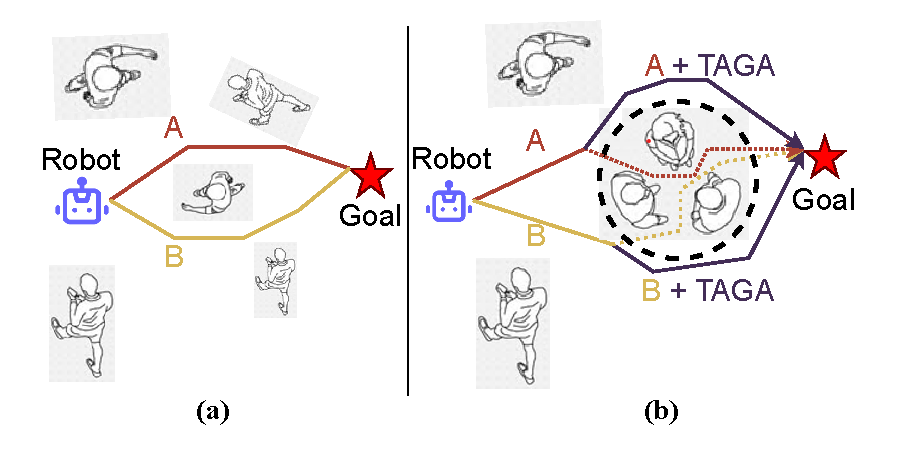
\includegraphics[width=4in]{figures/theme.pdf}
% \vspace{-23pt}
% \caption{\SR{Comparison of robot navigation with and without TAGA integration. (a) Traditional environment without group modeling, where robots navigate toward goals without considering human group formations. (b) Our enhanced environment with human groups (bounded by dotted black circles). Existing navigation frameworks (labeled A and B) frequently intrude into these groups, while their TAGA-enhanced versions (A+TAGA and B+TAGA) generate paths that respect group boundaries while maintaining effective navigation toward goals.}
% % (a) The figure represents the previous existing environment, which does not include human groups or defined boundaries. (b) In contrast, our modified environment introduces extended human groups, with group boundaries indicated by dotted black circles. Existing navigation frameworks like A and B struggle to adapt to group behaviors and often cross these boundaries. However, when our modular TAGA model is integrated with A and B, it effectively adapts to group behaviors, enabling appropriate interactions and crossings while respecting group boundaries.
% }
% The modified simulation environment used in this study. The figure shows a robot navigating towards a goal while predicting human positions. Humans within the robot’s observation area influence its trajectory, whereas those outside do not. The model considers both individual humans and human groups for socially aware navigation.
% \vspace{-15pt} 
% \label{fig-env-theme}
% \end{figure}

% In real-world crowded environments, people naturally form dynamic groups that move together, interact, and collectively influence navigation patterns \cite{moussaid2010walking}. Traditional approaches, such as reaction-based methods like Optimal Reciprocal Collision Avoidance (ORCA) \cite{orca} and Social Force (SF) \cite{helbing1995social}, as well as learning-based models \cite{liu2020decentralized, liu2023intention}, generally treat humans as separate individuals, failing to capture group-level interactions. As a result, robots relying on these methods may exhibit inefficient or socially inappropriate behaviors, such as cutting through groups rather than respecting their collective behaviors.

% Recently, a study \cite{group-aware} attempted to address this issue by introducing a group-aware policy for robot navigation, representing human groups using convex hulls and modeling them as pedestrians moving in the same direction. While their approach improves social compliance by discouraging the robot from intruding into groups, it lacks adaptability in mixed environments, as it primarily focuses on groups while overlooking individual interactions and more structured formations, such as static groups. 

% To overcome these limitations, we introduce human group modeling within a robot navigation framework utilizing the simulation environment from \cite{liu2023intention}, enabling robots to interact with both individual humans and human group behaviors (See Fig. \ref{fig-env-theme}). Additionally, we propose Tangent Action for Group Avoidance (TAGA), a reactive group-aware navigation model that dynamically adjusts robot trajectories based on detected human groups. Unlike previous approaches that rely solely on learned policies, TAGA provides a flexible avoidance mechanism that can be integrated into existing navigation methods, allowing these methods to adapt to group behaviors when human groups are present.

%To systematically evaluate the effectiveness of our approach, we conducted extensive experiments in diverse crowd settings. 
% Our study makes the following contributions:

% \begin{enumerate}
%     \item We developed an enhanced simulation framework that models both individual human dynamics and group behaviors with spatial clustering and leader-follower dynamics. This environment enables the evaluation of navigation strategies in complex crowd scenarios with diverse group formations.
    
    
%     % \item We developed an enhanced simulation framework that realistically models both individual human dynamics and human group behaviors, incorporating spatial clustering, leader-follower dynamics, and group boundary recognition. This environment enables the systematic evaluation of navigation strategies in complex crowd scenarios with diverse group formations.
    
%     \item We proposed TAGA, a reactive-based group avoidance mechanism that can be integrated into any robot navigation framework, allowing robots to dynamically adapt to human group behaviors and navigate in a socially compliant manner.
    
%     \item We introduced a new evaluation metric, Group Collision Rate (GCR), which quantifies how well a robot avoids intruding into human groups, providing a standardized approach to measure group-aware navigation performance.
    
%     \item We conducted a comprehensive benchmarking study by integrating TAGA with existing methods, including ORCA \cite{orca}, SF \cite{helbing1995social}, DS-RNN \cite{liu2020decentralized}, and AG-RL \cite{liu2023intention}, demonstrating significant improvements in group-aware navigation while maintaining comparable performance in other metrics.

%     \end{enumerate}

% \begin{enumerate}
%     \item \UT{We developed an advanced robot crowd interaction simulation environment that not only allows for the interaction of individual humans with the robot but also models dynamic human groups, providing a more realistic and comprehensive platform for evaluating navigation strategies in complex crowd scenarios.}
%     \item  We proposed a reactive-based group avoidance mechanism that can be integrated into any robot navigation framework, allowing robots to dynamically adapt to human group behaviors and navigate in a socially compliant manner.
%     \item To evaluate our model, we conducted a comprehensive benchmarking study by integrating TAGA with existing methods, including ORCA \cite{orca}, Social Force (SF) \cite{helbing1995social}, Decentralized Structural-RNN (DS-RNN) \cite{liu2020decentralized}, and Attention-Graph RL  (AG-RL) \cite{liu2023intention} Navigation models, to assess its impact on navigation performance. Additionally, to quantify group-aware navigation performance, we introduced a new evaluation metric, Group Collision Rate (GCR), which measures how well a robot avoids intruding into human groups.
% \end{enumerate}
% 1) We developed a robot crowd interaction simulation environment, where both individual humans and human groups can interact with the robot. This environment enables evaluating navigation strategies in realistic crowd scenarios.  
% 2) We proposed a reactive-based group avoidance mechanism that can be integrated into any robot navigation framework, allowing robots to dynamically adapt to human group behaviors and navigate in a socially compliant manner.  
% 3) To evaluate our model, we conducted a comprehensive benchmarking study by integrating TAGA with existing methods, including ORCA \cite{orca}, Social Force (SF) \cite{helbing1995social}, Decentralized Structural-RNN (DS-RNN) \cite{liu2020decentralized}, and Attention-Graph RL  (AG-RL) \cite{liu2023intention} Navigation models, to assess its impact on navigation performance. Additionally, to quantify group-aware navigation performance, we introduced a new evaluation metric, Group Collision Rate (GCR), which measures how well a robot avoids intruding into human groups.  


% Autonomous robots are increasingly being used in human environments for various applications, including service robotics, delivery, and assistive technologies. A growing number of research has focused on developing human-aware robot navigation by accounting for the fast and dynamic nature of human motion while adhering to complex social norms \cite{CHARALAMPOUS201785, pandey2017mobile, KRUSE20131726}. Early studies approached this problem by treating humans as moving obstacles to avoid \cite{fox1997dynamic}, designing strategies to prevent robots from getting stuck in crowds \cite{trautman2015robot}, and incorporating social norms to enable socially appropriate navigation \cite{robicquet2016learning, bera2017sociosense}. However, most of these methods have modeled humans as independent individuals, without considering the impact of groups on navigation.

% In real-world crowded environments, people naturally form dynamic groups that move together, interact, and collectively influence navigation patterns. Traditional approaches, such as reaction-based methods like Optimal Reciprocal Collision Avoidance (ORCA) \cite{orca} and Social Force (SF) \cite{helbing1995social}, as well as learning-based models \cite{liu2020decentralized, liu2023intention}, generally treat humans as separate individuals, failing to capture group-level interactions. As a result, robots relying on these methods may exhibit inefficient or socially inappropriate behaviors, such as cutting through groups rather than respecting their collective behaviors.

% Recently, a study \cite{group-aware} addressed this issues and introduced a group-aware policy for robot navigation by representing human groups using convex hulls and modeling them as pedestrians moving in the same direction. While their approach improves social compliance by discouraging the robot from intruding into groups, it lacks adaptability in mixed environments, as it primarily focuses on groups while overlooking individual interactions and more structured formations, such as static groups. 
% % Furthermore, their method relies solely on a learned policy, limiting real-time adaptability in complex scenarios.

% In this study, we address these limitations by introducing human group modeling within a robot navigation framework utilizing the simulation environment from \cite{liu2023intention}, enabling robots to interact with both individual humans and human group behaviors. Additionally, we propose TAGA, a reactive group-aware navigation model that dynamically adjusts robot trajectories based on detected human groups. TAGA provides a flexible avoidance mechanism that can be integrated into existing navigation approaches, allowing these methods to adapt to human group behaviors when a human group is detected.

% In this study, we address these limitations by introducing human group modeling within a robot navigation framework utilizing the simulation environment from \cite{liu2023intention}, enabling robots to interact with both individual humans and human groups. Additionally, we propose TAGA, a reactive group-aware navigation model that dynamically adjusts robot trajectories based on detected human groups. TAGA provides a flexible avoidance mechanism that can be integrated into existing navigation approaches, allowing these methods to adapt to group behaviors when human groups are present.

% Our study makes the following contributions.  
% 1) We developed a robot crowd interaction simulation environment, where both individual humans and human groups can interact with the robot. This environment enables evaluating navigation strategies in realistic crowd scenarios.  
% 2) We proposed a reactive-based group avoidance mechanism that can be integrated into any robot navigation framework, allowing robots to dynamically adapt to human group behaviors and navigate in a socially compliant manner.  
% 3) To evaluate our model, we conducted a comprehensive benchmarking study against ORCA \cite{orca}, Social Force (SF) \cite{helbing1995social}, DS-RNN \cite{liu2020decentralized}, and Intention-Aware Navigation (IAN) \cite{liu2023intention}. Additionally, to quantify group-aware navigation performance, we introduced a new evaluation metric, Group Collision Rate (GCR), which measures how well a robot avoids intruding into human groups.
% Unlike previous approaches that rely purely on learned policies, TAGA integrates a tangent-based avoidance mechanism, allowing real-time adaptability. 
% Furthermore, we introduce a new performance metric, Group Collision Rate (GCR), to quantitatively assess how well a robot avoids intruding into human groups.


% To evaluate our approach, we conduct a comprehensive benchmarking study against widely used navigation models, including ORCA \cite{orca}, SF \cite{helbing1995social}, DS-RNN \cite{liu2020decentralized}, and Intention-Aware Navigation (IAN) \cite{liu2023intention}. These methods primarily focus on individual human interactions, lacking explicit mechanisms for handling groups. By extending their frameworks to incorporate human group modeling, we assess their effectiveness in dense social settings. Our results demonstrate that TAGA significantly reduces group intrusions while maintaining competitive navigation efficiency compared to state-of-the-art baselines.
% Our study makes the following contributions.  
% 1) We developed a robot crowd interaction simulation environment, where both individual humans and human groups can interact with the robot. This environment enables evaluating navigation strategies in realistic crowd scenarios.  
% 2) We proposed a reactive-based group avoidance mechanism that can be integrated into any robot navigation framework, allowing robots to dynamically adapt to human group behaviors and navigate in a socially compliant manner.  
% 3) To evaluate our model, we conducted a comprehensive benchmarking study against ORCA \cite{orca}, Social Force (SF) \cite{helbing1995social}, DS-RNN \cite{liu2020decentralized}, and Intention-Aware Navigation (IAN) \cite{liu2023intention}. Additionally, to quantify group-aware navigation performance, we introduced a new evaluation metric, Group Collision Rate (GCR), which measures how well a robot avoids intruding into human groups.






% This template provides authors with most of the formatting specifications needed for preparing electronic versions of their papers. All standard paper components have been specified for three reasons: (1) ease of use when formatting individual papers, (2) automatic compliance to electronic requirements that facilitate the concurrent or later production of electronic products, and (3) conformity of style throughout a conference proceedings. Margins, column widths, line spacing, and type styles are built-in; examples of the type styles are provided throughout this document and are identified in italic type, within parentheses, following the example. Some components, such as multi-leveled equations, graphics, and tables are not prescribed, although the various table text styles are provided. The formatter will need to create these components, incorporating the applicable criteria that follow \cite{liu2020decentralized, liu2023intention}





